\section{Bearer-Authentication}
\label{clientbearerauth}

\subsection{Allgemeines}

Um die aktuell verfügbaren Menüs und Produkte sowie die Bestellungen eines Nutzers per API-Request
abfragen zu können, wird ein \textit{Bearer-Authorization-Token} benötigt.

\subsection{Generieren eines Bearer-Tokens}

Dieser setzt sich aus der E-Mail-Adresse des Nutzers und dem Token der aktuellen
Nutzer-Session zusammen.

\begin{code}[H]
    \centering
    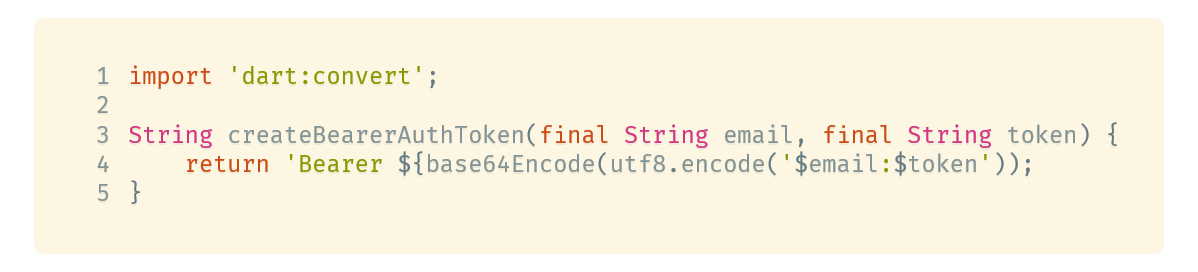
\includegraphics[width=1\textwidth]{images/Client/services/bearer-auth/generateBearerToken.png}
    \vspace{-25pt}
    \caption{Generieren eines Bearer-Authorizaton-Tokens}
\end{code}

\newpage

Rufen wir testweise oben angeführte Funktion auf,

\begin{code}[H]
    \centering
    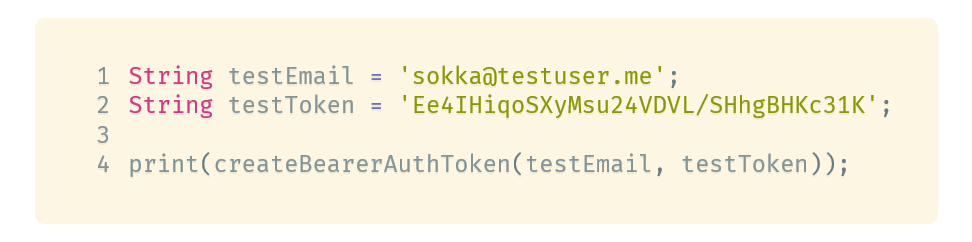
\includegraphics[width=1\textwidth]{images/Client/services/bearer-auth/callGenerateBearerToken.png}
    \vspace{-25pt}
    \caption{Erstellen eines Test-Bearer-Tokens}
\end{code}

erhalten wir folgenden Authorization-Token:

\begin{code}[H]
    \centering
    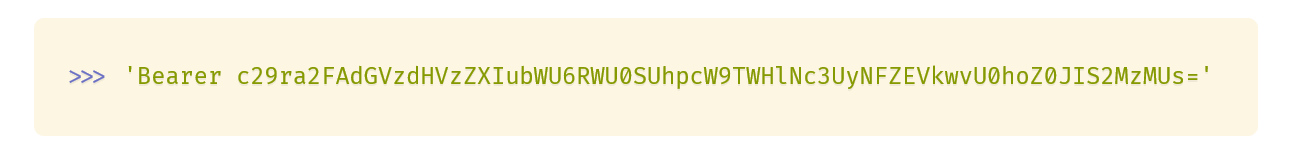
\includegraphics[width=1\textwidth]{images/Client/services/bearer-auth/testToken.png}
    \vspace{-25pt}
    \caption{Test-Bearer-Authorization-Token}
\end{code}

Ein solcher Token wird als \lstinline{Authorization}-Parameter bei Requests des \lstinline{FetchOrderables}-
oder des \lstinline{ManageOrders}-Service benötigt.